% Figure "column" of "Galashin's Conjecture 4.3 via a convex gradient": one column m of the necklace exponent matrix M_N,
% its cyclic difference Dm, the reading P_f D m at the rows s_x, and the column of B, for the window (3,5,1,2,4)
% (columns j=2, the edge 2->3, and j=7, the edge 5->2; CLH-2). Source in the paper's own fonts at the text width
% (6.5in = 468bp). It adds no assertion.
% Every value drawn is read from these Lean output lines (integer matrices; evaluated by Conj43.Eval):
%   S2EX02 s_x (x=1..n)=[3, 4, 1, 5, 2]
%   S2EX02 edgeOf j (j=1..columns, paper labels)=[(1, 2), (2, 3), (2, 4), (3, 5), (4, 5), (5, 1), (5, 2)]
%   EX02 M, S2EX02 D*M, EX02 P*D*M, EX02 B  (7 columns each; EX02 PDM=B : true)
% Build: pdflatex <this file> && pdftocairo -svg <this file>.pdf <this file>.svg
\documentclass[11pt]{standalone}
\usepackage[T1]{fontenc}
\usepackage{lmodern}
\usepackage{amsmath,amssymb}
\usepackage{tikz}
\usetikzlibrary{arrows.meta,positioning,calc}

% the palette of the paper's other figures: blue solid for the first strand, cycle or arc, ochre dashed for the second
\definecolor{ink}{HTML}{233740}
\definecolor{muted}{HTML}{65757D}
\definecolor{pblue}{HTML}{0072B2}
\definecolor{qochre}{HTML}{B87827}

\tikzset{
  base/.style={draw=muted, line width=0.5pt},
  ttl/.style={font=\small, text=ink, inner sep=0pt},
  lab/.style={font=\footnotesize, inner sep=1.2pt, text=ink},
  labm/.style={font=\small, inner sep=1.2pt, text=ink},
  labP/.style={font=\small, inner sep=1.2pt, text=pblue},
  labQ/.style={font=\small, inner sep=1.2pt, text=qochre},
  idx/.style={font=\footnotesize, text=muted, inner sep=0pt},
  negE/.style={font=\small, text=pblue, inner sep=0pt},
  posE/.style={font=\small, text=qochre, inner sep=0pt},
  zeroE/.style={font=\small, text=muted, inner sep=0pt},
  vtx/.style={circle, draw=ink, fill=white, line width=0.6pt, inner sep=0pt, minimum size=16bp, font=\small, text=ink},
  cycP/.style={pblue, line width=1.1pt, -{Stealth[length=5pt,width=4.2pt]}, shorten >=1pt, shorten <=1pt},
  cycQ/.style={qochre, line width=1.1pt, dash pattern=on 4pt off 1.6pt, -{Stealth[length=5pt,width=4.2pt]}, shorten >=1pt, shorten <=1pt},
  chord/.style={pblue, line width=0.9pt},
  arrP/.style={pblue, line width=1.0pt, -{Stealth[length=4.4pt,width=3.8pt]}},
  arrQ/.style={qochre, line width=1.0pt, dash pattern=on 4pt off 1.6pt, -{Stealth[length=4.4pt,width=3.8pt]}},
  arrM/.style={muted, line width=0.6pt, -{Stealth[length=4pt,width=3.4pt]}},
}

\begin{document}
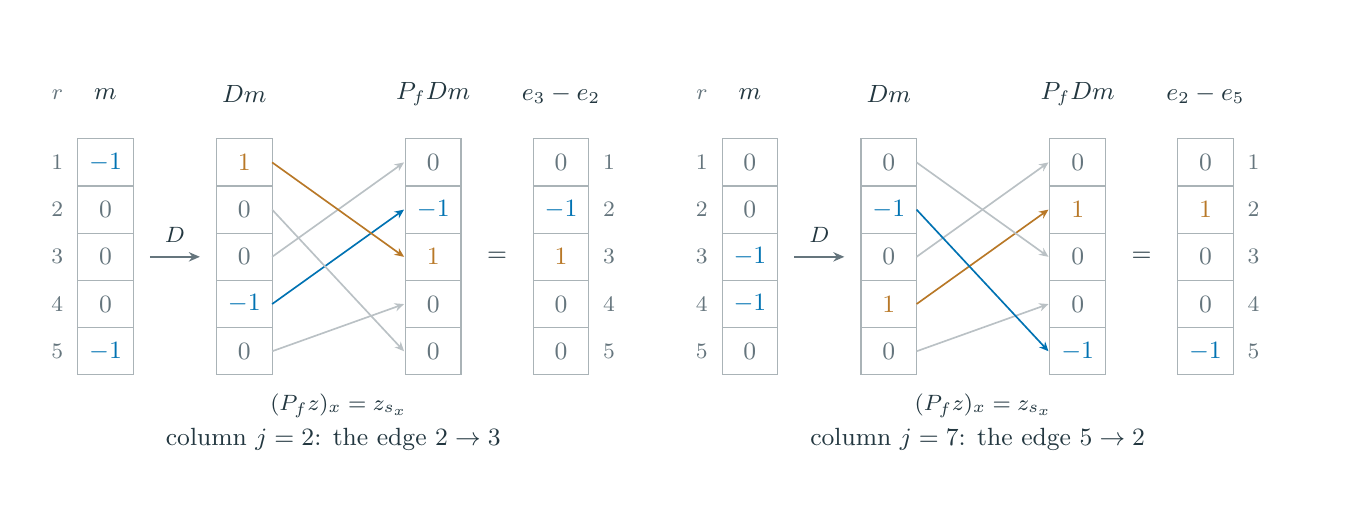
\begin{tikzpicture}[x=1bp,y=1bp]
\useasboundingbox (0,0) rectangle (468.000,168.000); %@ col canvas w=468.000 h=168.000
\node[labm] at (28.000,144.000) {$m$}; %@ col j=2 head c=0
\node[labm] at (78.000,144.000) {$Dm$}; %@ col j=2 head c=1
\node[labm] at (146.000,144.000) {$P_fDm$}; %@ col j=2 head c=2
\node[labm] at (192.000,144.000) {$e_3-e_2$}; %@ col j=2 head c=3
\draw[base, draw=muted!55, line width=0.4pt] (18.000,128.000) rectangle (38.000,111.000);
\node[negE] at (28.000,119.500) {$-1$}; %@ col j=2 cell stage=m row=1 val=-1
\draw[base, draw=muted!55, line width=0.4pt] (18.000,111.000) rectangle (38.000,94.000);
\node[zeroE] at (28.000,102.500) {$0$}; %@ col j=2 cell stage=m row=2 val=0
\draw[base, draw=muted!55, line width=0.4pt] (18.000,94.000) rectangle (38.000,77.000);
\node[zeroE] at (28.000,85.500) {$0$}; %@ col j=2 cell stage=m row=3 val=0
\draw[base, draw=muted!55, line width=0.4pt] (18.000,77.000) rectangle (38.000,60.000);
\node[zeroE] at (28.000,68.500) {$0$}; %@ col j=2 cell stage=m row=4 val=0
\draw[base, draw=muted!55, line width=0.4pt] (18.000,60.000) rectangle (38.000,43.000);
\node[negE] at (28.000,51.500) {$-1$}; %@ col j=2 cell stage=m row=5 val=-1
\draw[base, draw=muted!55, line width=0.4pt] (68.000,128.000) rectangle (88.000,111.000);
\node[posE] at (78.000,119.500) {$1$}; %@ col j=2 cell stage=Dm row=1 val=1
\draw[base, draw=muted!55, line width=0.4pt] (68.000,111.000) rectangle (88.000,94.000);
\node[zeroE] at (78.000,102.500) {$0$}; %@ col j=2 cell stage=Dm row=2 val=0
\draw[base, draw=muted!55, line width=0.4pt] (68.000,94.000) rectangle (88.000,77.000);
\node[zeroE] at (78.000,85.500) {$0$}; %@ col j=2 cell stage=Dm row=3 val=0
\draw[base, draw=muted!55, line width=0.4pt] (68.000,77.000) rectangle (88.000,60.000);
\node[negE] at (78.000,68.500) {$-1$}; %@ col j=2 cell stage=Dm row=4 val=-1
\draw[base, draw=muted!55, line width=0.4pt] (68.000,60.000) rectangle (88.000,43.000);
\node[zeroE] at (78.000,51.500) {$0$}; %@ col j=2 cell stage=Dm row=5 val=0
\draw[base, draw=muted!55, line width=0.4pt] (136.000,128.000) rectangle (156.000,111.000);
\node[zeroE] at (146.000,119.500) {$0$}; %@ col j=2 cell stage=PDm row=1 val=0
\draw[base, draw=muted!55, line width=0.4pt] (136.000,111.000) rectangle (156.000,94.000);
\node[negE] at (146.000,102.500) {$-1$}; %@ col j=2 cell stage=PDm row=2 val=-1
\draw[base, draw=muted!55, line width=0.4pt] (136.000,94.000) rectangle (156.000,77.000);
\node[posE] at (146.000,85.500) {$1$}; %@ col j=2 cell stage=PDm row=3 val=1
\draw[base, draw=muted!55, line width=0.4pt] (136.000,77.000) rectangle (156.000,60.000);
\node[zeroE] at (146.000,68.500) {$0$}; %@ col j=2 cell stage=PDm row=4 val=0
\draw[base, draw=muted!55, line width=0.4pt] (136.000,60.000) rectangle (156.000,43.000);
\node[zeroE] at (146.000,51.500) {$0$}; %@ col j=2 cell stage=PDm row=5 val=0
\draw[base, draw=muted!55, line width=0.4pt] (182.000,128.000) rectangle (202.000,111.000);
\node[zeroE] at (192.000,119.500) {$0$}; %@ col j=2 cell stage=B row=1 val=0
\draw[base, draw=muted!55, line width=0.4pt] (182.000,111.000) rectangle (202.000,94.000);
\node[negE] at (192.000,102.500) {$-1$}; %@ col j=2 cell stage=B row=2 val=-1
\draw[base, draw=muted!55, line width=0.4pt] (182.000,94.000) rectangle (202.000,77.000);
\node[posE] at (192.000,85.500) {$1$}; %@ col j=2 cell stage=B row=3 val=1
\draw[base, draw=muted!55, line width=0.4pt] (182.000,77.000) rectangle (202.000,60.000);
\node[zeroE] at (192.000,68.500) {$0$}; %@ col j=2 cell stage=B row=4 val=0
\draw[base, draw=muted!55, line width=0.4pt] (182.000,60.000) rectangle (202.000,43.000);
\node[zeroE] at (192.000,51.500) {$0$}; %@ col j=2 cell stage=B row=5 val=0
\node[idx,anchor=east] at (13.000,144.000) {$r$};
\node[idx,anchor=east] at (13.000,119.500) {$1$}; %@ col j=2 ridx r=1
\node[idx,anchor=west] at (207.000,119.500) {$1$}; %@ col j=2 xidx x=1
\node[idx,anchor=east] at (13.000,102.500) {$2$}; %@ col j=2 ridx r=2
\node[idx,anchor=west] at (207.000,102.500) {$2$}; %@ col j=2 xidx x=2
\node[idx,anchor=east] at (13.000,85.500) {$3$}; %@ col j=2 ridx r=3
\node[idx,anchor=west] at (207.000,85.500) {$3$}; %@ col j=2 xidx x=3
\node[idx,anchor=east] at (13.000,68.500) {$4$}; %@ col j=2 ridx r=4
\node[idx,anchor=west] at (207.000,68.500) {$4$}; %@ col j=2 xidx x=4
\node[idx,anchor=east] at (13.000,51.500) {$5$}; %@ col j=2 ridx r=5
\node[idx,anchor=west] at (207.000,51.500) {$5$}; %@ col j=2 xidx x=5
\draw[arrM] (44.000,85.500) -- (62.000,85.500);
\node[lab] at (53.000,93.500) {$D$};
\draw[muted!45, line width=0.6pt, -{Stealth[length=3.4pt,width=3pt]}] (88.000,85.500) -- (135.500,119.500); %@ col j=2 link x=1 s=3
\draw[pblue, line width=0.6pt, -{Stealth[length=3.4pt,width=3pt]}] (88.000,68.500) -- (135.500,102.500); %@ col j=2 link x=2 s=4
\draw[qochre, line width=0.6pt, -{Stealth[length=3.4pt,width=3pt]}] (88.000,119.500) -- (135.500,85.500); %@ col j=2 link x=3 s=1
\draw[muted!45, line width=0.6pt, -{Stealth[length=3.4pt,width=3pt]}] (88.000,51.500) -- (135.500,68.500); %@ col j=2 link x=4 s=5
\draw[muted!45, line width=0.6pt, -{Stealth[length=3.4pt,width=3pt]}] (88.000,102.500) -- (135.500,51.500); %@ col j=2 link x=5 s=2
\node[lab] at (112.000,32.000) {$(P_fz)_x=z_{s_x}$};
\node[labm] at (169.000,85.500) {$=$};
\node[labm] at (110.000,20.000) {column $j=2$: the edge $2\to3$}; %@ col j=2 caption p=2 q=3
\node[labm] at (260.000,144.000) {$m$}; %@ col j=7 head c=0
\node[labm] at (310.000,144.000) {$Dm$}; %@ col j=7 head c=1
\node[labm] at (378.000,144.000) {$P_fDm$}; %@ col j=7 head c=2
\node[labm] at (424.000,144.000) {$e_2-e_5$}; %@ col j=7 head c=3
\draw[base, draw=muted!55, line width=0.4pt] (250.000,128.000) rectangle (270.000,111.000);
\node[zeroE] at (260.000,119.500) {$0$}; %@ col j=7 cell stage=m row=1 val=0
\draw[base, draw=muted!55, line width=0.4pt] (250.000,111.000) rectangle (270.000,94.000);
\node[zeroE] at (260.000,102.500) {$0$}; %@ col j=7 cell stage=m row=2 val=0
\draw[base, draw=muted!55, line width=0.4pt] (250.000,94.000) rectangle (270.000,77.000);
\node[negE] at (260.000,85.500) {$-1$}; %@ col j=7 cell stage=m row=3 val=-1
\draw[base, draw=muted!55, line width=0.4pt] (250.000,77.000) rectangle (270.000,60.000);
\node[negE] at (260.000,68.500) {$-1$}; %@ col j=7 cell stage=m row=4 val=-1
\draw[base, draw=muted!55, line width=0.4pt] (250.000,60.000) rectangle (270.000,43.000);
\node[zeroE] at (260.000,51.500) {$0$}; %@ col j=7 cell stage=m row=5 val=0
\draw[base, draw=muted!55, line width=0.4pt] (300.000,128.000) rectangle (320.000,111.000);
\node[zeroE] at (310.000,119.500) {$0$}; %@ col j=7 cell stage=Dm row=1 val=0
\draw[base, draw=muted!55, line width=0.4pt] (300.000,111.000) rectangle (320.000,94.000);
\node[negE] at (310.000,102.500) {$-1$}; %@ col j=7 cell stage=Dm row=2 val=-1
\draw[base, draw=muted!55, line width=0.4pt] (300.000,94.000) rectangle (320.000,77.000);
\node[zeroE] at (310.000,85.500) {$0$}; %@ col j=7 cell stage=Dm row=3 val=0
\draw[base, draw=muted!55, line width=0.4pt] (300.000,77.000) rectangle (320.000,60.000);
\node[posE] at (310.000,68.500) {$1$}; %@ col j=7 cell stage=Dm row=4 val=1
\draw[base, draw=muted!55, line width=0.4pt] (300.000,60.000) rectangle (320.000,43.000);
\node[zeroE] at (310.000,51.500) {$0$}; %@ col j=7 cell stage=Dm row=5 val=0
\draw[base, draw=muted!55, line width=0.4pt] (368.000,128.000) rectangle (388.000,111.000);
\node[zeroE] at (378.000,119.500) {$0$}; %@ col j=7 cell stage=PDm row=1 val=0
\draw[base, draw=muted!55, line width=0.4pt] (368.000,111.000) rectangle (388.000,94.000);
\node[posE] at (378.000,102.500) {$1$}; %@ col j=7 cell stage=PDm row=2 val=1
\draw[base, draw=muted!55, line width=0.4pt] (368.000,94.000) rectangle (388.000,77.000);
\node[zeroE] at (378.000,85.500) {$0$}; %@ col j=7 cell stage=PDm row=3 val=0
\draw[base, draw=muted!55, line width=0.4pt] (368.000,77.000) rectangle (388.000,60.000);
\node[zeroE] at (378.000,68.500) {$0$}; %@ col j=7 cell stage=PDm row=4 val=0
\draw[base, draw=muted!55, line width=0.4pt] (368.000,60.000) rectangle (388.000,43.000);
\node[negE] at (378.000,51.500) {$-1$}; %@ col j=7 cell stage=PDm row=5 val=-1
\draw[base, draw=muted!55, line width=0.4pt] (414.000,128.000) rectangle (434.000,111.000);
\node[zeroE] at (424.000,119.500) {$0$}; %@ col j=7 cell stage=B row=1 val=0
\draw[base, draw=muted!55, line width=0.4pt] (414.000,111.000) rectangle (434.000,94.000);
\node[posE] at (424.000,102.500) {$1$}; %@ col j=7 cell stage=B row=2 val=1
\draw[base, draw=muted!55, line width=0.4pt] (414.000,94.000) rectangle (434.000,77.000);
\node[zeroE] at (424.000,85.500) {$0$}; %@ col j=7 cell stage=B row=3 val=0
\draw[base, draw=muted!55, line width=0.4pt] (414.000,77.000) rectangle (434.000,60.000);
\node[zeroE] at (424.000,68.500) {$0$}; %@ col j=7 cell stage=B row=4 val=0
\draw[base, draw=muted!55, line width=0.4pt] (414.000,60.000) rectangle (434.000,43.000);
\node[negE] at (424.000,51.500) {$-1$}; %@ col j=7 cell stage=B row=5 val=-1
\node[idx,anchor=east] at (245.000,144.000) {$r$};
\node[idx,anchor=east] at (245.000,119.500) {$1$}; %@ col j=7 ridx r=1
\node[idx,anchor=west] at (439.000,119.500) {$1$}; %@ col j=7 xidx x=1
\node[idx,anchor=east] at (245.000,102.500) {$2$}; %@ col j=7 ridx r=2
\node[idx,anchor=west] at (439.000,102.500) {$2$}; %@ col j=7 xidx x=2
\node[idx,anchor=east] at (245.000,85.500) {$3$}; %@ col j=7 ridx r=3
\node[idx,anchor=west] at (439.000,85.500) {$3$}; %@ col j=7 xidx x=3
\node[idx,anchor=east] at (245.000,68.500) {$4$}; %@ col j=7 ridx r=4
\node[idx,anchor=west] at (439.000,68.500) {$4$}; %@ col j=7 xidx x=4
\node[idx,anchor=east] at (245.000,51.500) {$5$}; %@ col j=7 ridx r=5
\node[idx,anchor=west] at (439.000,51.500) {$5$}; %@ col j=7 xidx x=5
\draw[arrM] (276.000,85.500) -- (294.000,85.500);
\node[lab] at (285.000,93.500) {$D$};
\draw[muted!45, line width=0.6pt, -{Stealth[length=3.4pt,width=3pt]}] (320.000,85.500) -- (367.500,119.500); %@ col j=7 link x=1 s=3
\draw[qochre, line width=0.6pt, -{Stealth[length=3.4pt,width=3pt]}] (320.000,68.500) -- (367.500,102.500); %@ col j=7 link x=2 s=4
\draw[muted!45, line width=0.6pt, -{Stealth[length=3.4pt,width=3pt]}] (320.000,119.500) -- (367.500,85.500); %@ col j=7 link x=3 s=1
\draw[muted!45, line width=0.6pt, -{Stealth[length=3.4pt,width=3pt]}] (320.000,51.500) -- (367.500,68.500); %@ col j=7 link x=4 s=5
\draw[pblue, line width=0.6pt, -{Stealth[length=3.4pt,width=3pt]}] (320.000,102.500) -- (367.500,51.500); %@ col j=7 link x=5 s=2
\node[lab] at (344.000,32.000) {$(P_fz)_x=z_{s_x}$};
\node[labm] at (401.000,85.500) {$=$};
\node[labm] at (342.000,20.000) {column $j=7$: the edge $5\to2$}; %@ col j=7 caption p=5 q=2
\end{tikzpicture}
\end{document}
